\documentclass[11pt,letterpaper]{article}

\usepackage[margin=2.35cm,headheight=15pt]{geometry}
\usepackage[T1]{fontenc}
\usepackage{lmodern}
\usepackage[spanish,es-nodecimaldot]{babel}
\usepackage{graphicx}
\usepackage{booktabs}
\usepackage{tabularx}
\usepackage{array}
\usepackage{xcolor}
\usepackage{listings}
\usepackage{fancyhdr}
\usepackage{titlesec}
\usepackage{enumitem}
\usepackage{hyperref}
\usepackage{caption}
\usepackage{float}

\definecolor{RoadGreen}{HTML}{164B3B}
\definecolor{RoadTeal}{HTML}{197A89}
\definecolor{RoadBlue}{HTML}{245A8D}
\definecolor{RoadRed}{HTML}{C9364C}
\definecolor{RoadLight}{HTML}{EDF4F0}
\definecolor{RoadGray}{HTML}{53665F}
\definecolor{CodeBack}{HTML}{F4F7F5}
\definecolor{CodeBorder}{HTML}{B8C9C1}

\hypersetup{
  colorlinks=true,
  linkcolor=RoadBlue,
  urlcolor=RoadTeal,
  pdftitle={Proyecto de Sistemas Embebidos: Módulo celular},
  pdfauthor={Roderic David Munguia Calvillo}
}

\pagestyle{fancy}
\fancyhf{}
\fancyhead[L]{\small\sffamily RoadLink}
\fancyhead[R]{\small\sffamily Módulo celular}
\fancyfoot[C]{\small\sffamily\thepage}
\renewcommand{\headrulewidth}{0.4pt}
\renewcommand{\headrule}{\hbox to\headwidth{\color{RoadTeal}\leaders\hrule height \headrulewidth\hfill}}

\titleformat{\section}{\Large\bfseries\sffamily\color{RoadGreen}}{\thesection}{0.7em}{}
\titleformat{\subsection}{\large\bfseries\sffamily\color{RoadTeal}}{\thesubsection}{0.7em}{}
\titlespacing*{\section}{0pt}{2.2ex plus 0.8ex}{1.0ex}
\titlespacing*{\subsection}{0pt}{1.7ex plus 0.5ex}{0.7ex}

\setlist[itemize]{leftmargin=1.5em,itemsep=0.25em,topsep=0.35em}
\setlist[enumerate]{leftmargin=1.7em,itemsep=0.3em,topsep=0.35em}
\renewcommand{\arraystretch}{1.22}
\newcolumntype{Y}{>{\raggedright\arraybackslash}X}
\emergencystretch=1.5em

\lstdefinestyle{roadcode}{
  language=C++,
  backgroundcolor=\color{CodeBack},
  frame=single,
  rulecolor=\color{CodeBorder},
  basicstyle=\ttfamily\footnotesize,
  keywordstyle=\color{RoadBlue}\bfseries,
  stringstyle=\color{RoadRed},
  commentstyle=\color{RoadGray}\itshape,
  numbers=left,
  numberstyle=\scriptsize\color{RoadGray},
  numbersep=8pt,
  showstringspaces=false,
  breaklines=true,
  columns=fullflexible,
  keepspaces=true
}

\newcommand{\rutaimagenes}{../../recursos/imagenes/}
\newcommand{\fotomodulo}[3]{%
  \begin{figure}[H]
    \centering
    \IfFileExists{\rutaimagenes#1}{%
      \includegraphics[width=0.82\textwidth,height=7cm,keepaspectratio]{\rutaimagenes#1}%
    }{%
      \fcolorbox{RoadTeal}{RoadLight}{%
        \begin{minipage}[c][5.0cm][c]{0.82\textwidth}
          \centering
          {\Large\sffamily\bfseries\color{RoadGreen} Fotografía pendiente}\par\vspace{0.45em}
          {\sffamily #2}\par\vspace{0.55em}
          {\small\sffamily Archivo requerido: \texttt{\detokenize{#1}}}
        \end{minipage}}%
    }
    \caption{#3}
  \end{figure}
}

\begin{document}

\begin{titlepage}
  \pagecolor{RoadLight}
  \begin{center}
    \vspace*{1.0cm}
    {\sffamily\bfseries\fontsize{20}{24}\selectfont\color{RoadTeal} ROADLINK}\par
    \vspace{0.35cm}
    {\color{RoadTeal}\rule{0.82\textwidth}{2.2pt}}\par
    \vfill
    {\sffamily\bfseries\fontsize{28}{34}\selectfont\color{RoadGreen} Proyecto de Sistemas Embebidos}\par
    \vspace{0.35cm}
    {\sffamily\bfseries\fontsize{38}{44}\selectfont\color{RoadBlue} Módulo celular}\par
    \vspace{0.8cm}
    \vfill
    \begin{tabular}{>{\sffamily\bfseries}r >{\sffamily}l}
      Autor: & Roderic David Munguia Calvillo \\
      Proyecto: & RoadLink \\
      Fecha: & 16 de septiembre de 2026 \\
    \end{tabular}
    \vfill
    \begin{minipage}{0.82\textwidth}
      \centering
      \colorbox{RoadGreen}{\parbox{0.94\textwidth}{\centering\color{white}\sffamily\small
        Documentación del módulo de comunicación celular}}
    \end{minipage}
    \vspace*{0.8cm}
  \end{center}
\end{titlepage}
\nopagecolor

\pagenumbering{roman}
\tableofcontents
\clearpage
\pagenumbering{arabic}

\section{Introducción}

RoadLink comenzó con la idea de desarrollar un sistema de monitoreo económico y flexible para vehículos comerciales, principalmente
(\textit{machine-to-machine}, M2M). La primera fase no fue conectar de inmediato
todos los subsistemas del vehículo, sino evaluar el principal objetivo: que un
microcontrolador (ESP32) pudiera preparar información y enviarla de manera autónoma a
través de una red celular.

Aprovechando módulos económicos y con documentación extensa, se utilizó
un ESP32 conectado únicamente a un módulo SIM800L. Los datos enviados eran
simulados, por lo que todavía no dependían del bus CAN, del GPS ni de la interfaz
gráfica de RoadLink. La primera evidencia de comunicación se obtuvo mediante un
SMS. Posteriormente, el desarrollo avanzó hacia el uso de una conexión de datos
y el envío de información por Internet.

La evolución del proyecto llevó a sustituir el SIM800L por un A7670SA como
plataforma celular de la versión actual, principalmente por la disminución del soporte de las compañías celulares para la red 2G. El cambio conserva el mismo concepto
general: el ESP32 reúne los datos, controla el módulo SIM mediante comandos AT por
UART y entrega un paquete de datos a una computadora remota.

\section{Objetivo}

El objetivo del subsistema celular es permitir que RoadLink transmita
información del vehículo hacia un destino externo, sin depender de una conexión
local. Para esto se evaluaron los siguientes objetivos:

\begin{itemize}
  \item establecer comunicación serial confiable entre el ESP32 y el módem;
  \item verificar la tarjeta SIM, el registro en la red y la calidad de señal;
  \item mandar datos reales de GPS y OBD-II a un servidor o computadora central;
  \item detectar errores, aplicar tiempos límite y reintentar sin bloquear el sistema;
  \item separar la alimentación del módulo celular del microcontrolador ESP32;
  \item conservar una interfaz de software y hardware que permita cambiar el módulo celular sin rediseñar RoadLink completo.
\end{itemize}

Este documento se centra en la primera fase del proyecto que fue probar el concepto de enviar datos remotamente a través de una red celular.

\section{Evolución del desarrollo}

\begin{table}[H]
  \centering
  \caption{Etapas principales del subsistema celular.}
  \begin{tabularx}{\textwidth}{>{\bfseries\raggedright\arraybackslash}p{3.3cm} Y Y}
    \toprule
    Etapa & Propósito & Resultado dentro del proyecto \\
    \midrule
    \shortstack[l]{Prueba\\básica} & Confirmar UART y respuesta a comandos AT & El ESP32 puede controlar el módem y leer sus respuestas. \\
    \shortstack[l]{SMS con\\SIM800L} & Demostrar comunicación M2M con datos simulados & Un destino externo recibe un mensaje generado automáticamente. \\
    \shortstack[l]{Datos por\\Internet} & Sustituir el mensaje manual por telemetría estructurada & Se define el uso de una carga JSON y una entrega HTTP. \\
    \shortstack[l]{Integración\\A7670SA} & Actualizar la plataforma celular conservando la arquitectura & El nuevo módem se integra como transporte celular de RoadLink. \\
    \bottomrule
  \end{tabularx}
\end{table}

La tabla anterior resume las pruebas principales de esta fase del proyecto y el orden en que se realizaron.

\section{Arquitectura del subsistema}

La Figura~\ref{fig:arquitectura-celular} muestra las conexiones de forma simplificada. La
entrada del sistema alimenta dos convertidores reductores. Una salida se reserva
para el módulo SIM y la otra alimenta la electrónica lógica. Este diseño permite intercambiar fácilmente entre distintos módulos SIM, así como aislar las fuentes de alimentación (véase la Sección~\ref{sec:alimentacion}).
El enlace UART entre el ESP32 y el módulo SIM se realizaba a través de un reductor de voltaje en la primera versión con el módulo SIM800L; sin embargo, con el nuevo módulo 4G A7670SA es directo, ya que opera con el mismo nivel de voltaje lógico de 3.3 V que el ESP32.

\subsection{Criterios de diseño}

La distribución mantiene rutas funcionales fáciles de seguir y aplica cuatro
criterios principales:

\begin{itemize}
  \item alimentación celular independiente de la alimentación lógica;
  \item tierra común para conservar la referencia eléctrica de UART;
  \item adaptación de niveles entre el controlador y el módem (primera versión, no directa);
  \item separación entre adquisición de datos y transporte celular.
\end{itemize}

\subsection{Funciones de cada módulo}

\begin{table}[H]
  \centering
  \caption{Responsabilidad de los bloques principales.}
  \begin{tabularx}{\textwidth}{>{\bfseries\raggedright\arraybackslash}p{4.1cm} Y}
    \toprule
    Módulo & Función \\
    \midrule
    ESP32 & Ejecuta el firmware, reúne telemetría, construye mensajes y controla el módem. \\
    SIM800L & Plataforma 2G de las primeras pruebas de SMS y comunicación de datos. \\
    A7670SA & Plataforma celular 4G utilizada en la integración actual de RoadLink. \\
    \shortstack[l]{Alimentación\\celular} & Fuente separada capaz de responder a los picos de consumo del módem. \\
    \shortstack[l]{Alimentación\\lógica} & Fuente para el ESP32 y la electrónica de control. \\
    \bottomrule
  \end{tabularx}
\end{table}

\subsection{Capas de comunicación}

\begin{table}[H]
  \centering
  \caption{Protocolos y formato empleados por RoadLink.}
  \begin{tabularx}{\textwidth}{>{\bfseries\raggedright\arraybackslash}p{3.0cm} >{\raggedright\arraybackslash}p{3.2cm} Y}
    \toprule
    Capa & Tecnología & Uso en RoadLink \\
    \midrule
    Enlace local & UART & Comandos AT, respuestas y datos entre ESP32 y módem. \\
    Control del módem & Comandos AT & Registro, señal, contexto de datos y transmisión. \\
    Red móvil & Datos por paquetes & Transporte desde el módem hacia Internet. \\
    Aplicación & HTTP POST & Entrega de telemetría al recurso \texttt{/telemetry}. \\
    Contenido & JSON & Datos GPS, OBD-II, estado y clave de acceso. \\
    \bottomrule
  \end{tabularx}
\end{table}

\begin{figure}[H]
  \centering
  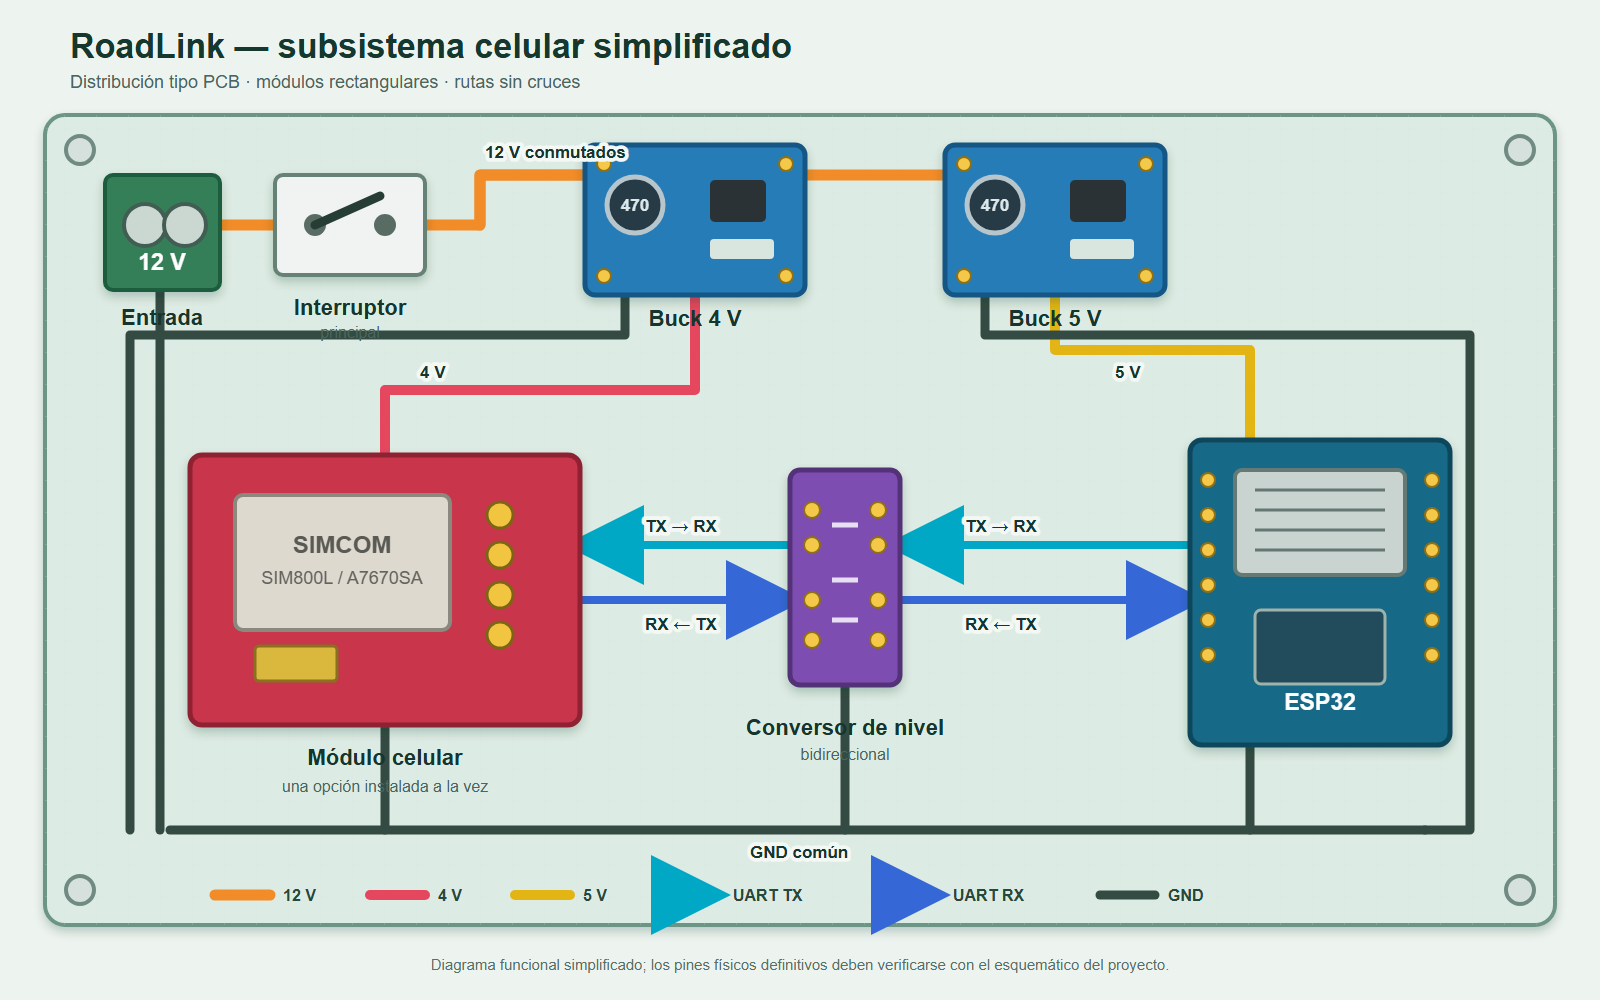
\includegraphics[width=0.75\textwidth]{../../recursos/imagenes/esquema-celular-simplificado.png}
  \caption{Arquitectura simplificada de alimentación y comunicación celular.}
  \label{fig:arquitectura-celular}
\end{figure}

\section{Primera etapa: prueba con SIM800L}

El SIM800L se utilizó inicialmente como un módulo independiente del resto de
RoadLink. El ESP32 generaba valores simulados, preparaba un mensaje y controlaba
el módem mediante comandos AT. Esta configuración demostró la capacidad M2M sin
necesitar todavía una conexión al vehículo.

\fotomodulo{sim800l-modulo.jpg}{Módulo SIM800L utilizado en las primeras pruebas del proyecto.}{Módulo SIM800L utilizado durante la primera etapa de desarrollo.}

\subsection{Prueba básica de SMS}

La prueba utiliza el modo de texto del módem. El siguiente código muestra la
secuencia mínima y utiliza nombres simbólicos para los pines y el número de
destino.

\begin{lstlisting}[style=roadcode,caption={Código básico para una prueba de SMS.}]
HardwareSerial modem(1);

void setup() {
  modem.begin(MODEM_BAUD, SERIAL_8N1, MODEM_RX, MODEM_TX);
  delay(1000);

  modem.println("AT");
  delay(500);
  modem.println("AT+CMGF=1");          // SMS en modo texto
  delay(500);
  modem.println("AT+CMGS=\"NUMERO_DESTINO\"");
  delay(500);
  modem.print("RoadLink: prueba M2M correcta");
  modem.write(26);                     // Ctrl+Z: enviar
}
\end{lstlisting}

Una prueba completa también debe leer las respuestas, confirmar \texttt{OK},
detectar errores y limitar los tiempos de espera.

\subsection{Criterios de validación}

\begin{enumerate}
  \item El módem responde al comando \texttt{AT}.
  \item La tarjeta SIM está disponible y el módem se registra en la red.
  \item El mensaje se envía sin reinicios causados por la alimentación.
  \item El teléfono de prueba recibe exactamente el texto generado por el ESP32.
  \item El monitor serial conserva el intercambio como evidencia.
\end{enumerate}

\fotomodulo{esp32-sim800l-montaje-prueba.jpg}{ESP32, fuente de alimentación y SIM800L utilizados en la prueba inicial.}{Montaje de la primera prueba M2M con SIM800L.}

\section{Integración actual con A7670SA}

En la etapa actual, el A7670SA cumple la función de transporte celular de
RoadLink. El cambio de módulo no modifica el formato recibido por el servidor. Sin embargo, este nuevo módulo ofrece mayor ancho de banda y disponibilidad de redes para la conectividad.

\fotomodulo{a7670sa-modulo.jpg}{Módulo A7670SA utilizado en la integración actual.}{Módulo A7670SA utilizado durante la etapa actual de desarrollo.}

El firmware organiza este proceso como una máquina de estados no bloqueante.
Esto es importante porque una operación celular puede tardar varios segundos.

\subsection{Conexión lógica con el firmware}

El código existente inicializa el servicio celular con su UART, señales de
control y parámetros guardados. Después, llama al método de actualización en
cada vuelta del programa principal:

\begin{lstlisting}[style=roadcode,caption={Integración no bloqueante del servicio celular.}]
sim.begin(
    AppConfig::SIM_BAUD,
    Pins::SIM_RX, Pins::SIM_TX, Pins::SIM_RST,
    settings.simEnabled, settings.simAutoSend,
    settings.simSendGps, settings.simSendObd,
    settings.simSendIntervalMs,
    settings.simServerIp, settings.simServerPort,
    settings.simAccessKey);

void loop() {
  sim.update();
}
\end{lstlisting}


\subsection{Flujo de transmisión}

\begin{enumerate}
  \item iniciar UART y aplicar la secuencia de encendido o reinicio;
  \item comprobar comunicación básica mediante \texttt{AT};
  \item verificar la tarjeta SIM, el registro y la calidad de señal;
  \item activar el contexto de datos de la red móvil;
  \item construir una carga JSON con la información seleccionada;
  \item realizar una solicitud HTTP POST hacia \texttt{/telemetry};
  \item registrar el código HTTP y reintentar si ocurre una falla.
\end{enumerate}

El siguiente extracto muestra la intención del envío HTTP sin reproducir la
máquina de estados completa:

\begin{lstlisting}[style=roadcode,caption={Núcleo del envío HTTP del servicio celular.}]
startCommand("AT+HTTPINIT", timeout);
startCommand("AT+HTTPPARA=\"CID\",1", timeout);
startCommand("AT+HTTPPARA=\"CONTENT\",\"application/json\"", timeout);
startCommand(String("AT+HTTPDATA=") + payload.length() + ",10000", timeout);
serial.print(payload);
startCommand("AT+HTTPACTION=1", httpTimeout);  // POST
\end{lstlisting}

\subsection{Formato de la telemetría}

RoadLink transmite una estructura JSON. Los campos no disponibles se envían
como \texttt{null}; además, GPS y OBD-II pueden habilitarse por separado.

\begin{lstlisting}[style=roadcode,language={},caption={Ejemplo reducido de la carga útil JSON.}]
{
  "access_key": "123456",
  "device": "roadlink",
  "gps": {
    "valid": true,
    "latitude": 20.000000,
    "longitude": -103.000000
  },
  "obd": {
    "rpm": 1850,
    "speed_kmh": 43,
    "coolant_c": 91
  }
}
\end{lstlisting}

La dirección IP, el puerto y la clave se configuran en RoadLink y se conservan
en memoria no volátil. El servidor o la computadora de base valida la clave y registra la telemetría.

\fotomodulo{esp32-a7670sa-montaje-prueba.jpg}{ESP32, alimentación, conversor de nivel y A7670SA utilizados en la integración actual.}{Montaje de integración del A7670SA con RoadLink.}

\section{Alimentación eléctrica}\label{sec:alimentacion}

Un módulo celular puede producir cambios rápidos de corriente al registrarse o
transmitir. Una fuente inestable en reposo puede sufrir una caída de voltaje
durante esos eventos y provocar reinicios, pérdida de red o respuestas seriales
incompletas.

El diseño separa la alimentación celular de la alimentación lógica mediante
convertidores reductores. Las tierras permanecen unidas para proporcionar una
referencia común a UART.

Antes de energizar el montaje se debe verificar:

\begin{itemize}
  \item voltaje de entrada, polaridad y ajuste de cada convertidor;
  \item capacidad de corriente durante transmisión;
  \item continuidad de la tierra común;
  \item dirección de TX y RX;
  \item niveles lógicos permitidos por el hardware utilizado;
  \item conexión de antena antes del registro celular.
\end{itemize}

\section{Conclusiones}

El módulo celular de RoadLink siguió una progresión práctica. La prueba con
SIM800L y datos simulados confirmó la comunicación M2M por SMS. Después, la
solución evolucionó hacia datos estructurados enviados por Internet. Finalmente,
el A7670SA se incorporó como plataforma de la etapa actual sin modificar la
función central del sistema.

La arquitectura separa la adquisición de datos, el control del módem y el
receptor remoto. UART y los comandos AT mantienen una interfaz comprensible;
HTTP POST y JSON proporcionan un formato sencillo para transportar telemetría;
y la máquina de estados evita que los tiempos celulares detengan RoadLink.

Las siguientes mejoras documentales serán incorporar la fotografía individual
pendiente del A7670SA, resultados medidos y capturas de las pruebas. Estas evidencias permitirán
relacionar cada decisión de diseño con el prototipo físico.

\end{document}
